\documentclass[10pt,compress]{beamer} % Change 10pt to make fonts of a different size
\mode<presentation>

\usepackage[spanish]{babel}
\usepackage{fontspec}
\usepackage{tikz}
\usepackage{etoolbox}
\usepackage{xcolor}
\usepackage{xstring}
\usepackage{listings}

\usetheme{UAH}
\usecolortheme{UAH}
\setbeamertemplate{navigation symbols}{} 
\setbeamertemplate{caption}[numbered]

%%%%%%%%%%%%%%%%%%%%%%%%%%%%%%%%%%%%%%%%%%%%%%%%%%%%%%%%%%%%%%%%%
%% Presentation Info
\title[Codificación de Canal]{Codificación de Canal}
\author{Enrique Alexandre}
\institute{Dpto. de Teoría de la Señal y Comunicaciones}
\date{Curso 2020/2021}
%%%%%%%%%%%%%%%%%%%%%%%%%%%%%%%%%%%%%%%%%%%%%%%%%%%%%%%%%%%%%%%%%


%%%%%%%%%%%%%%%%%%%%%%%%%%%%%%%%%%%%%%%%%%%%%%%%%%%%%%%%%%%%%%%%%
%% Descomentar para habilitar barra de navegación superior
\setNavigation
%%%%%%%%%%%%%%%%%%%%%%%%%%%%%%%%%%%%%%%%%%%%%%%%%%%%%%%%%%%%%%%%%

%%%%%%%%%%%%%%%%%%%%%%%%%%%%%%%%%%%%%%%%%%%%%%%%%%%%%%%%%%%%%%%%%
%% Configuración de logotipos en portada
%% Opacidad de los logotipos
\newcommand{\opacidad}{1}
%%%%%%%%%%%%%%%%%%%%%%%%%%%%%%%%%%%%%%%%%%%%%%%%%%%%%%%%%%%%%%%%%

%%%%%%%%%%%%%%%%%%%%%%%%%%%%%%%%%%%%%%%%%%%%%%%%%%%%%%%%%%%%%%%%%
%% FOOTLINE
%% Comment/Uncomment the following blocks to modify the footline
%% content in the body slides. 
%% Option A: Title and institute
\footlineA
%%%%%%%%%%%%%%%%%%%%%%%%%%%%%%%%%%%%%%%%%%%%%%%%%%%%%%%%%%%%%%%%%

\begin{document}

%%%%%%%%%%%%%%%%%%%%%%%%%%%%%%%%%%%%%%%%%%%%%%%%%%%%%%%%%%%%%%%%%
% Use this block for a blue title slide with modified footline
{\titlepageBlue
    \begin{frame}
        \titlepage
    \end{frame}
}

{
\disableNavigation{white}
\begin{frame}[shrink]{Índice}
 \frametitle{Índice}
 \tableofcontents
  % You might wish to add the option [pausesections]
\end{frame}
}

\section{Introducción}

\subsection{Motivación}

\begin{frame}{Introducción}{Motivación}
    \begin{itemize}
		\item Existencia de canales ruidosos
		\begin{itemize}
			\item Necesidad de transmitir información libre de errores
		\end{itemize}
	\end{itemize}
	\centering 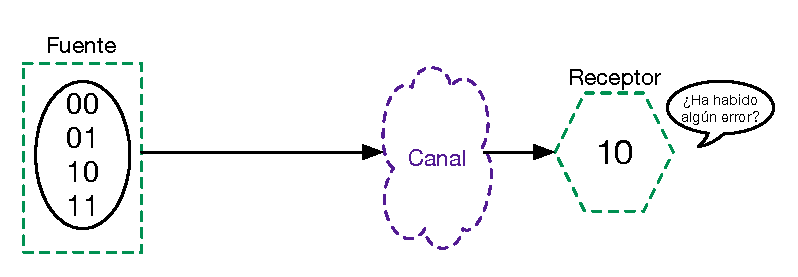
\includegraphics[width=0.7\linewidth]{Figuras/CodificacionDeCanal1.pdf}
	\centering 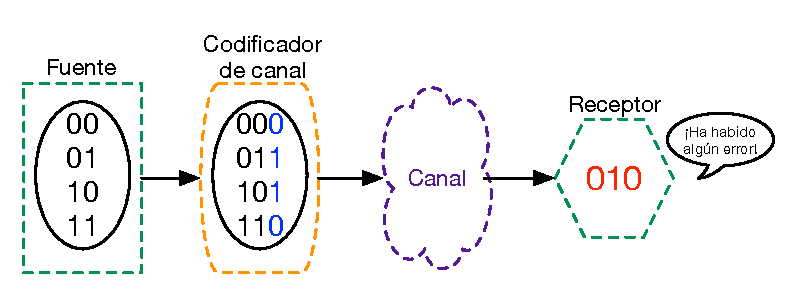
\includegraphics[width=0.7\linewidth]{Figuras/CodificacionDeCanal2.pdf}
\end{frame}

\subsection{Parámetros importantes}

\begin{frame}{Introducción}{Parámetros importantes}
  \begin{itemize}
    \item {\bf Tasa de codificación:} Relación entre el número de bits de información y el número de bits totales transmitidos.
    \item {\bf Distancia Hamming: }Número de elementos distintos entre dos vectores.
    \item {\bf Distancia mínima:} La menor distancia Hamming entre dos palabras código válidas.
  \end{itemize}
\end{frame}

\subsection{Detección y corrección de errores}
\begin{frame}{Introducción}{Detección y corrección de errores}
  \begin{itemize}
    \item Dado un código con una distancia mínima $d_{min}$:
    \begin{itemize}
      \item Se pueden {\bf detectar} $d_{min}-1$ errores.
      \item Se pueden {\bf corregir} $(d_{min}-1)/2$ errores.
    \end{itemize}
  \end{itemize}
\end{frame}

\subsection{¿Y la probabilidad de error?}
\begin{frame}{Introducción}{¿Y la probabilidad de error?}
  \begin{itemize}
    \item Supongamos que la probabilidad de error en un bit es $p_e$.
    \item La probabilidad de que ocurran $i$ errores en una palabra código con $n$ bits se puede calcular como:\\
    \begin{displaymath}
      p(i,n) = \binom{n}{i} \cdot P_e^i \cdot (1-p_e)^{n-i} \approx \binom{n}{i} \cdot p_e^i
    \end{displaymath}
    \ \\
    \begin{displaymath}
      \binom{n}{i} = \frac{n!}{i! (n-i)!}
    \end{displaymath}
  \end{itemize}
\end{frame}

\section{Códigos de repetición}

\subsection{Definición}
\begin{frame}{Códigos de repetición}{Definición}
	\begin{itemize}
		\item Posiblemente la solución más sencilla:
		\begin{itemize}
			\item Repito cada bit transmitido $n$ veces
		\end{itemize}
		\item Por ejemplo, si $n=3$:
	\end{itemize}
	\centering \includegraphics[width=0.8\linewidth]{Figuras/CodificacionDeRepetición.pdf}
\end{frame}

\subsection{Cálculo de la probabilidad de error}
\begin{frame}{Códigos de repetición}{Cálculo de la probabilidad de error}
\begin{itemize}
  \item Supongamos lo siguiente:
  \begin{itemize}
    \item $p_e = 10^{-6}$
    \item Código de repetición con $k=1$ y $n=3$.
  \end{itemize}
  \item La probabilidad de que haya algún error pero no lo detectemos será:
  \begin{displaymath}
    p(3,3) = p_e^3 = 10^{-18}
  \end{displaymath}
  \item La probabilidad de que haya algún error y no lo podamos corregir:
  \begin{displaymath}
    p = p(2,3) + p(3,3) = 3 \cdot p_e^2 - 2p_e^3 \approx 3 \cdot 10^{-12}
  \end{displaymath}
\end{itemize}
\end{frame}

\section{Códigos de paridad}
\begin{frame}{Códigos de paridad}
  \begin{itemize}
    \item Se utiliza $n = k+1$.
    \item El bit de paridad es tal que el número de unos en la palabra código sea par (paridad par) o impar (paridad impar).
  \end{itemize}
  \centering 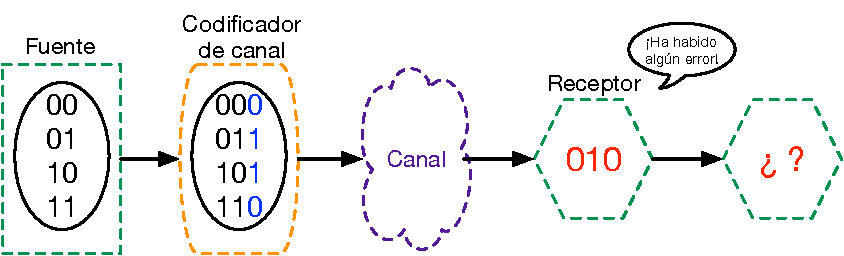
\includegraphics[width=0.8\linewidth]{Figuras/CodificacionDeparidad.pdf}
\end{frame}


\section{Códigos bloque}
\begin{frame}{Códigos bloque}
  \begin{itemize}
    \item En realidad agrupan también a los anteriores.
    \item Un par de definiciones:
    \begin{itemize}
      \item {\bf Código lineal:}
      \begin{itemize}
        \item La suma de dos vectores código es otro vector código.
        \item El vector $0$ forma parte del código.
      \end{itemize}
      \item {\bf Peso de un vector:}
      \begin{itemize}
        \item Es el número de unos que tiene el vector.
      \end{itemize}
      \item {\bf Distancia mínima:}
      \begin{itemize}
        \item Se puede calcular como el peso mínimo del código
      \end{itemize}
    \end{itemize}
  \end{itemize}
\end{frame}

\begin{frame}{Códigos bloque}
  \begin{itemize}
    \item Supongamos un mensaje a transmitir, $\mathbf{m} = (m_1, m_2, \cdots, m_k)$.
    \item Y el correspondiente vector transmitido: $\mathbf{x} = (x_1, x_2, \cdots, x_n)$.
    \item En un código bloque, ambos vectores se relacionan matricialmente como:
    \begin{displaymath}
      \mathbf{x} = \mathbf{m} \cdot \mathbf{G}
    \end{displaymath}
    \item Donde $\mathbf{G}$ es la {\bf matriz generadora} del código, de dimensiones $(k \times n)$.
    \item Decimos que un {\bf código es sistemático} si la matriz generadora es tal que:
    \begin{displaymath}
      \mathbf{G} = [ \mathbf{I_k} | \mathbf{P} ]
    \end{displaymath}
  \end{itemize}
\end{frame}

\begin{frame}{Códigos bloque}
  \begin{itemize}
    \item ¿Y cómo decodificamos el mensaje?
    \item Se utiliza la matriz de paridad $\mathbf{H}$, de dimensiones $(n-k \times n)$:
    \begin{displaymath}
      \mathbf{H} = [ \mathbf{P}^T | \mathbf{I_{n-k}}]
    \end{displaymath}
    \item Si recibimos un vector $\mathbf{y}$ (que en realidad será el vector transmitido $\mathbf{x}$ más ruido ($\mathbf{e}$), haremos lo siguiente:
    \begin{displaymath}
      \mathbf{s} = \mathbf{y} \cdot \mathbf{H}^T
    \end{displaymath}
    \item A $\mathbf{s}$ se le llama {\bf síndrome}, y si es nulo, la palabra código $\mathbf{y}$ es válida.
  \end{itemize}
\end{frame}

\begin{frame}{Códigos bloque}
  \begin{itemize}
    \item Y los errores, ¿cómo se corrigen?
    \item Es posible demostrar que el síndrome depende exclusivamente del error cometido ($\mathbf{e}$), y no del vector transmitido ($\mathbf{x}$).
    \item Pero hay un problema:
    \begin{itemize}
      \item Si $\mathbf{x}$ tiene $n$ bits, hay $2^n$ posibles vectores de error.
      \item El síndrome sólo tiene $n-k$ bits:
      \begin{itemize}
        \item Sólo hay $2^{n-k}$ síndromes posibles
      \end{itemize}
    \end{itemize}
  \end{itemize}
\end{frame}

\subsection{Decodificación de máxima verosimilitud}
\begin{frame}{Códigos bloque}{Decodificación de máxima verosimilitud}
  \begin{itemize}
    \item Creamos una tabla con los síndromes correspondientes a los $2^{n-k-1}$ vectores de error más probables.
    \item ¿Qué hará el decodificador?
    \begin{itemize}
      \item Calcula el síndrome: $\mathbf{s} = \mathbf{y} \cdot \mathbf{H}^T$
      \item Busca en la tabla ese síndrome
      \item Obtiene el vector de error correspondiente ($\mathbf{\hat{e}}$)
      \item Obtiene cuál sería la palabra decodificada: $\mathbf{y} + \mathbf{\hat{e}}$
    \end{itemize}
  \end{itemize}
\end{frame}

\subsection{Códigos Hamming}
\begin{frame}{Códigos bloque}{Códigos Hamming}
  \begin{itemize}
    \item No hemos visto cómo se define la matriz generadora de un código bloque.
    \item Hay muchos métodos, pero quizás el más conocido es el de {\bf códigos Hamming}.
    \item Se caracterizan por:
    \begin{itemize}
      \item Bits de control: $q = n - k \geq 3$.
      \item $n= 2^q - 1$
      \item Independientemente del valor de $q$, $d_{min}=3$:
      \begin{itemize}
        \item Podemos detectar hasta $2$ errores
        \item Podemos corregir hasta $1$ error.
      \end{itemize}
    \end{itemize}
  \end{itemize}
\end{frame}


\begin{frame}{Códigos bloque}{Códigos Hamming}
  \begin{itemize}
    \item Para crear la matriz de comprobación de paridad, colocamos todos los vectores binarios posibles en las columnas, ordenados de forma que quede la matriz identidad al final:
    \begin{displaymath}
      \mathbf{H} = \left [ \begin{array}{cccc}
      \mathtt{0} & \mathtt{1} & \mathtt{1} & \mathtt{1}\\
      \mathtt{1} & \mathtt{1} & \mathtt{0} & \mathtt{1}\\
      \mathtt{1} & \mathtt{0} & \mathtt{1} & \mathtt{1}\\ 	
     \end{array}
     \left |
      \begin{array}{ccc}
      \mathtt{1} & \mathtt{0} & \mathtt{0} \\
      \mathtt{0} & \mathtt{1} & \mathtt{0} \\
      \mathtt{0} & \mathtt{0} & \mathtt{1} \\
     \end{array}
     \right.
      \right ]
    \end{displaymath}
  \end{itemize}
\end{frame}


\begin{frame}{Códigos bloque}{Códigos Hamming}
  \begin{itemize}
    \item A partir de aquí, es inmediato calcular $\mathbf{G}$, sabiendo que $\mathbf{H} = [\mathbf{P}^T | \mathbf{I}_q ]$:
    \begin{displaymath}
      \mathbf{G} = \left [ \begin{array}{cccc}
      \mathtt{1} & \mathtt{0} & \mathtt{0} & \mathtt{0}\\
      \mathtt{0} & \mathtt{1} & \mathtt{0} & \mathtt{0}\\
      \mathtt{0} & \mathtt{0} & \mathtt{1} & \mathtt{0}\\
      \mathtt{0} & \mathtt{0} & \mathtt{0} & \mathtt{1}\\	 	
     \end{array}
     \left |
      \begin{array}{ccc}
      \mathtt{0} & \mathtt{1} & \mathtt{1} \\
      \mathtt{1} & \mathtt{1} & \mathtt{0} \\
      \mathtt{1} & \mathtt{0} & \mathtt{1} \\
      \mathtt{1} & \mathtt{1} & \mathtt{1} \\	 	
     \end{array}
     \right.
      \right ]
    \end{displaymath}
  \end{itemize}
\end{frame}


\section{Decodificación dura y blanda}
\subsection{Definición}

\begin{frame}{Decodificación dura y blanda}{Definición}
  \begin{itemize}
    \item {\bf Decodificación dura:}
    \begin{itemize}
      \item Es lo que hemos venido haciendo hasta ahora.
      \item La palabra recibida se decodifica bit a bit.
      \item Se elige aquella palabra código a una distancia Hamming menor.
    \end{itemize}
    \item {\bf Decodificación blanda:}
    \begin{itemize}
      \item En este caso se elige el símbolo a una menor distancia euclídea.
      \item La probabilidad de error va a ser menor
    \end{itemize}
  \end{itemize}
\end{frame}

\subsection{Ejemplo}
\begin{frame}{Decodificación dura y blanda}{Ejemplo}
  \begin{itemize}
    \item Supongamos lo siguiente: 
    \begin{itemize}
      \item Código de paridad con $n=3$.
      \item Utilizamos una modulación PAM unipolar con amplitudes $0V$ y $1V$.
      \item Suponemos además que:
      \begin{itemize}
        \item Se transmite el símbolo $\mathbf{011}$.
        \item Es decir, transmitimos por el canal la señal $0V - 1V - 1V$.
        \item En el receptor obtenemos: $0.2V - 0.45V - 0.7V$
      \end{itemize}
    \end{itemize}
  \end{itemize}
\end{frame}

\begin{frame}{Decodificación dura y blanda}{Ejemplo}
  \begin{itemize}
    \item Si utilizamos decodificación dura: 
    \begin{itemize}
      \item El receptor obtendrá:
      \begin{itemize}
        \item $0.2V \rightarrow 0$
        \item $0.45V \rightarrow 0$
        \item $0.7V \rightarrow 1$
      \end{itemize}
      \item Es decir, recibimos el vector $\mathbf{001}$, que sabemos que es incorrecto.
      \item Hay cuatro posibles palabras código: $\mathbf{000}$, $\mathbf{011}$, $\mathbf{101}$ y $\mathbf{110}$.
      \item Las distancias Hamming de nuestra palabra a cada una de éstas es: $1$, $1$, $1$ y $3$ respectivamente.
      \item Por tanto, elegiremos una de las tres primeras al azar.
      \item Y acertaremos {\bf 1 de cada 3 veces}.
    \end{itemize}
  \end{itemize}
\end{frame}


\begin{frame}{Decodificación dura y blanda}{Ejemplo}
  \begin{itemize}
    \item Si utilizamos decodificación blanda: 
    \begin{itemize}
      \item Recibimos el mismo vector que antes: $0.2V - 0.45V-0.7V$.
      \item En este caso calculamos la distancia euclídea desde este vector a cada uno de los posibles símbolos de mi constelación:
      \begin{itemize}
        \item $000 \rightarrow (0 - 0.2)^2 + (0-0.45)^2 + (0-0.7)^2 = 0.73$
        \item $011 \rightarrow (0 - 0.2)^2 + (1-0.45)^2 + (1-0.7)^2 = 0.43$
        \item $101 \rightarrow (1 - 0.2)^2 + (0-0.45)^2 + (1-0.7)^2 = 0.93$
        \item $110 \rightarrow (1 - 0.2)^2 + (1-0.45)^2 + (0-0.7)^2 = 1.43$
      \end{itemize}
      \item Finalmente elegiremos el símbolo $\mathbf{011}$.
    \end{itemize}
  \end{itemize}
\end{frame}

\section{Códigos convolucionales}
\subsection{Introducción}
\begin{frame}{Códigos convolucionales}{Introducción}
  \begin{itemize}
    \item Principal diferencia con lo anterior: tienen memoria
    \item Ejemplo: Código $(n,k,L) = (2,1,2)$.
  \end{itemize}
  \centering 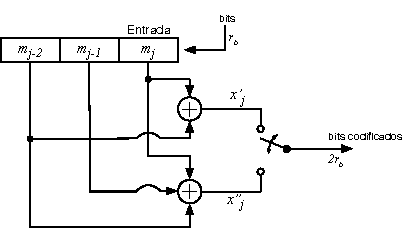
\includegraphics[width=0.8\linewidth]{Figuras/CodificadorConvolucional.pdf}
\end{frame}


\subsection{Árbol del código}
\begin{frame}{Códigos convolucionales}{Árbol del código}
  \centering 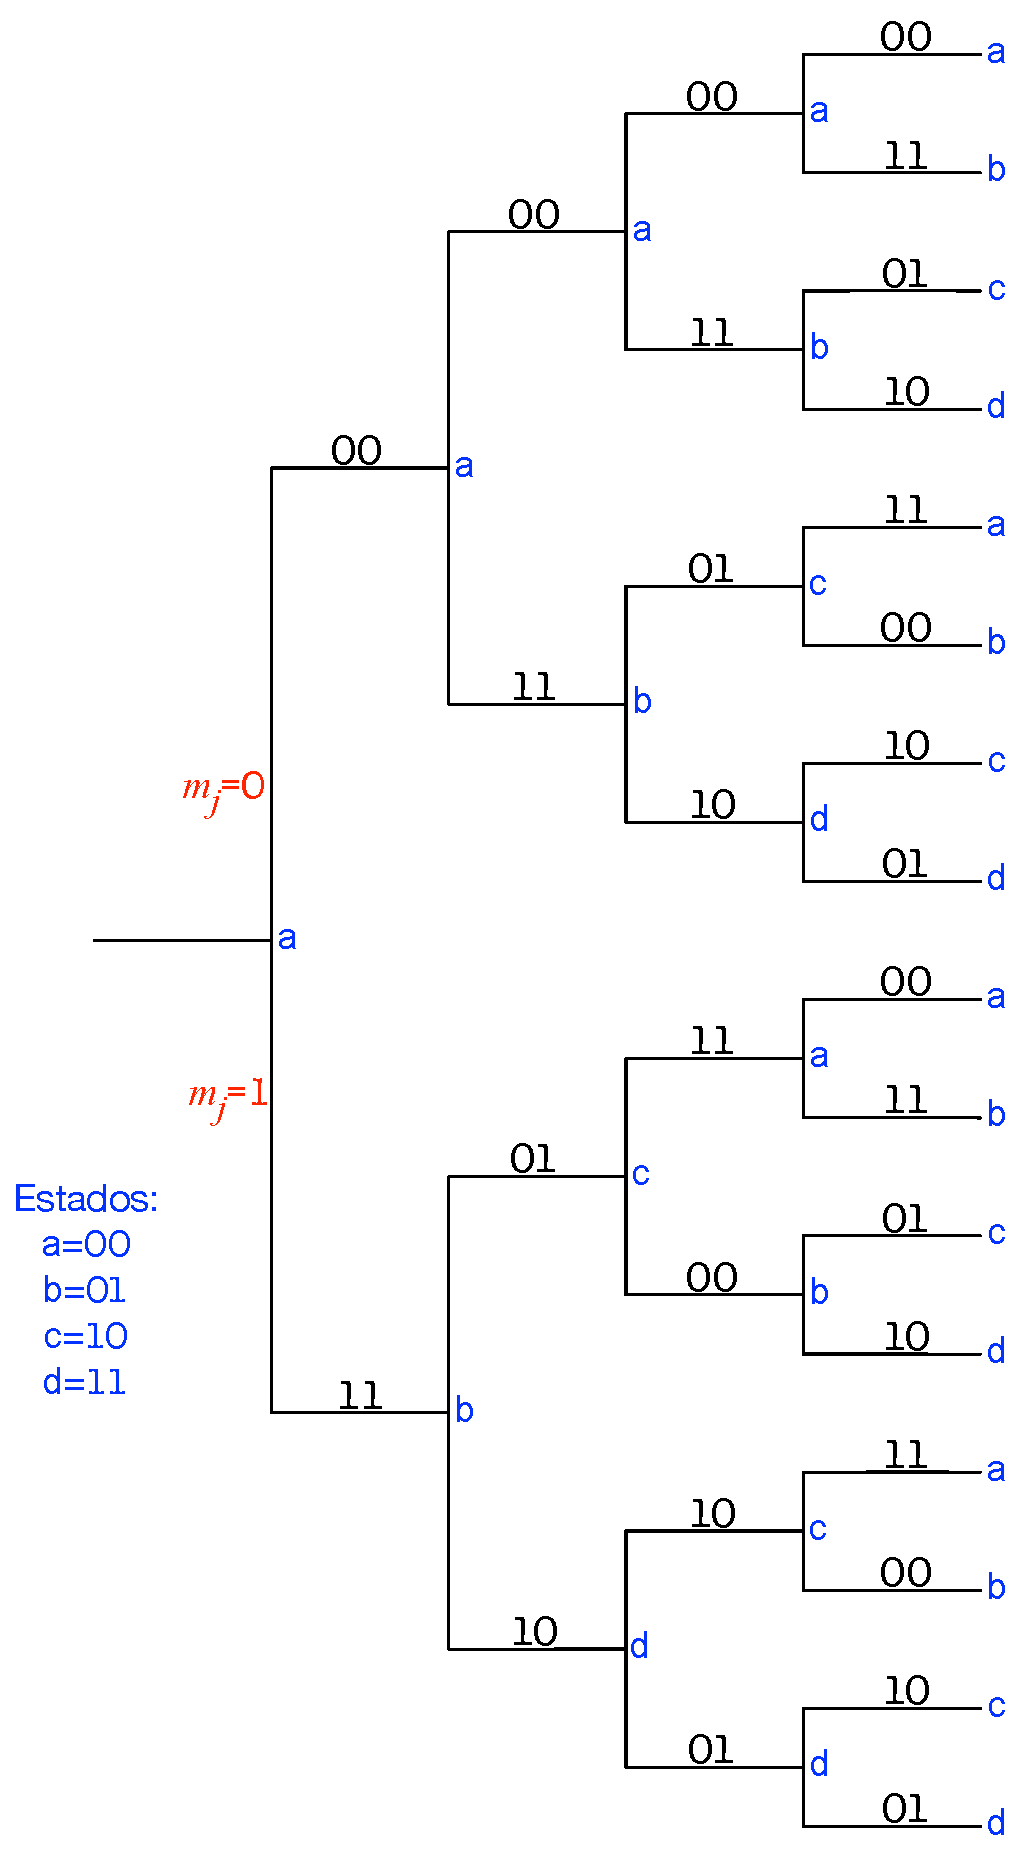
\includegraphics[width=0.33\linewidth]{Figuras/ArbolCodigoConvolucional.pdf}
\end{frame}

\subsection{Diagrama de rejilla}
\begin{frame}{Códigos convolucionales}{Diagrama de rejilla}
  \centering 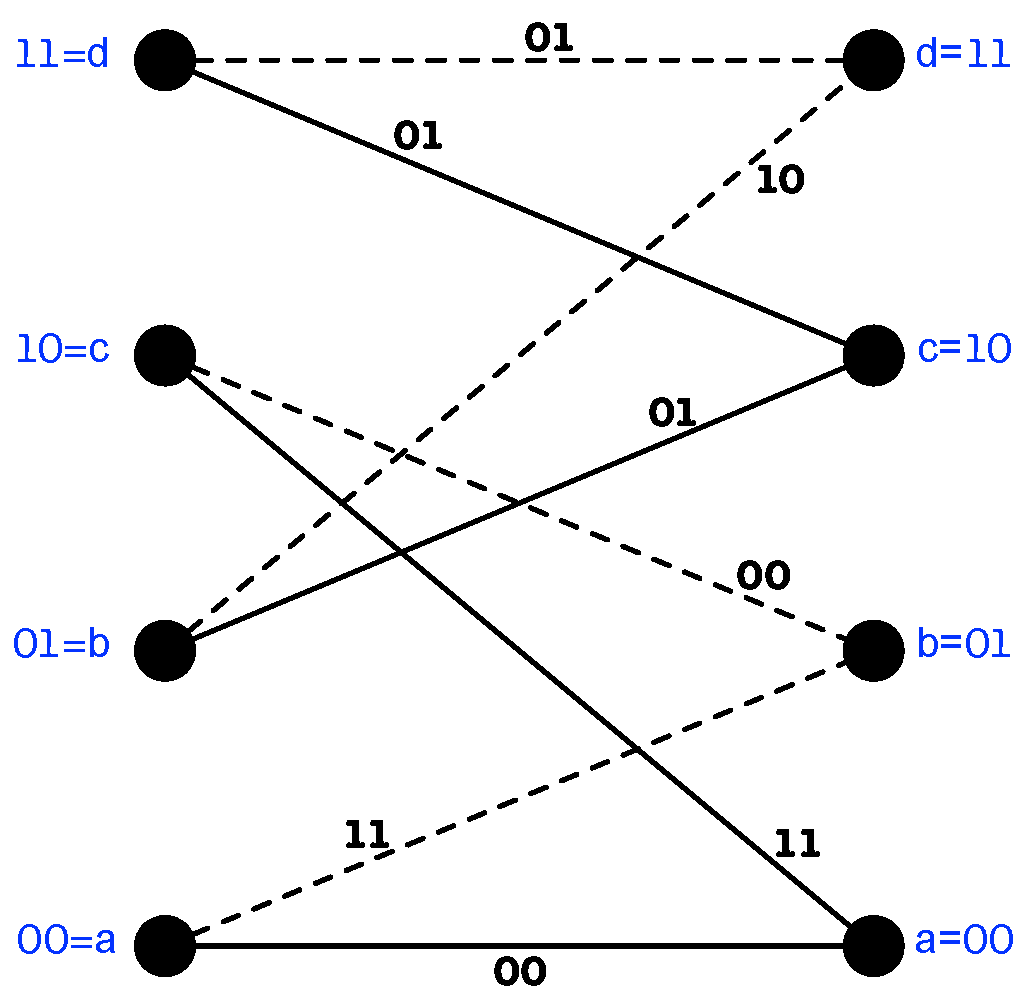
\includegraphics[width=0.6\linewidth]{Figuras/RejillaCodigoConvolucional2.pdf}
\end{frame}

\subsection{Diagrama de estados}
\begin{frame}{Códigos convolucionales}{Diagrama de estados}
  \centering 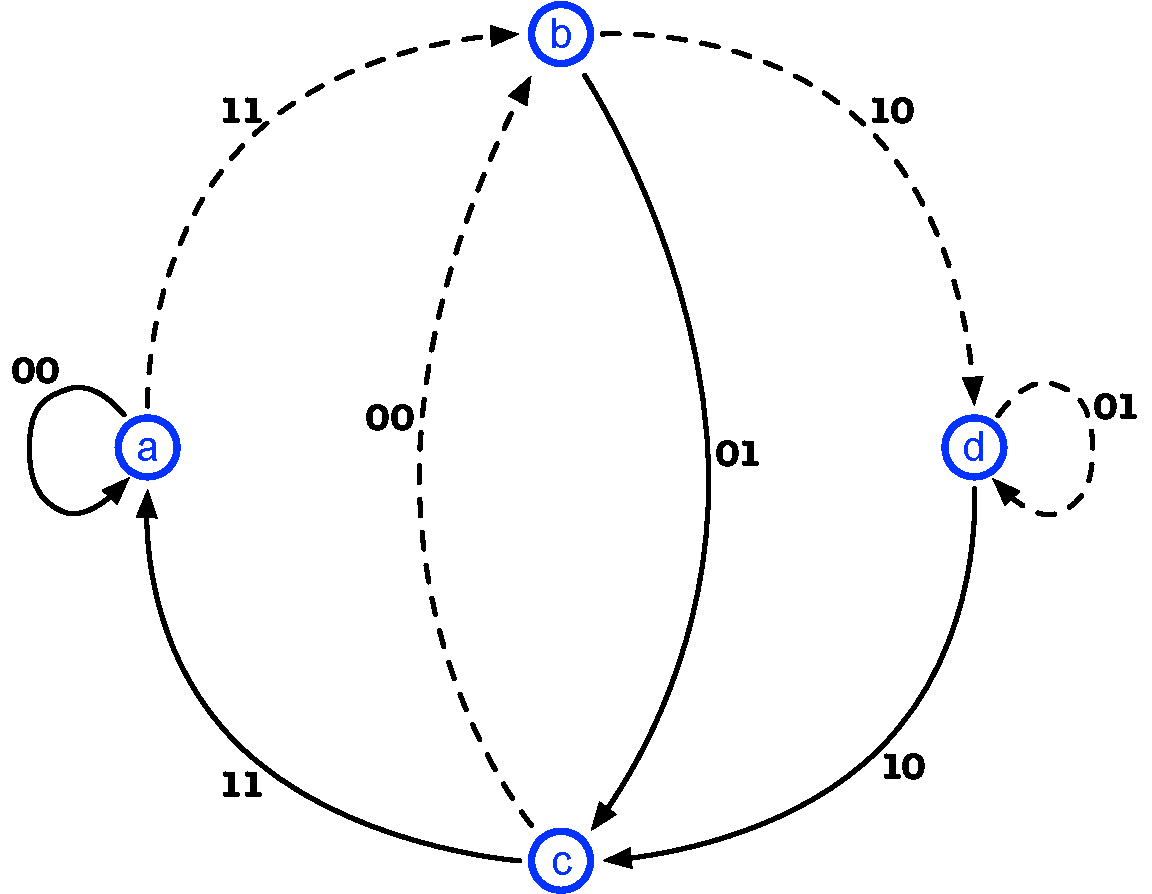
\includegraphics[width=0.6\linewidth]{Figuras/EstadosCodigoConvolucional.pdf}
\end{frame}

\subsection{Algoritmo de Viterbi}
\begin{frame}{Códigos convolucionales}{Algoritmo de Viterbi}
  \centering 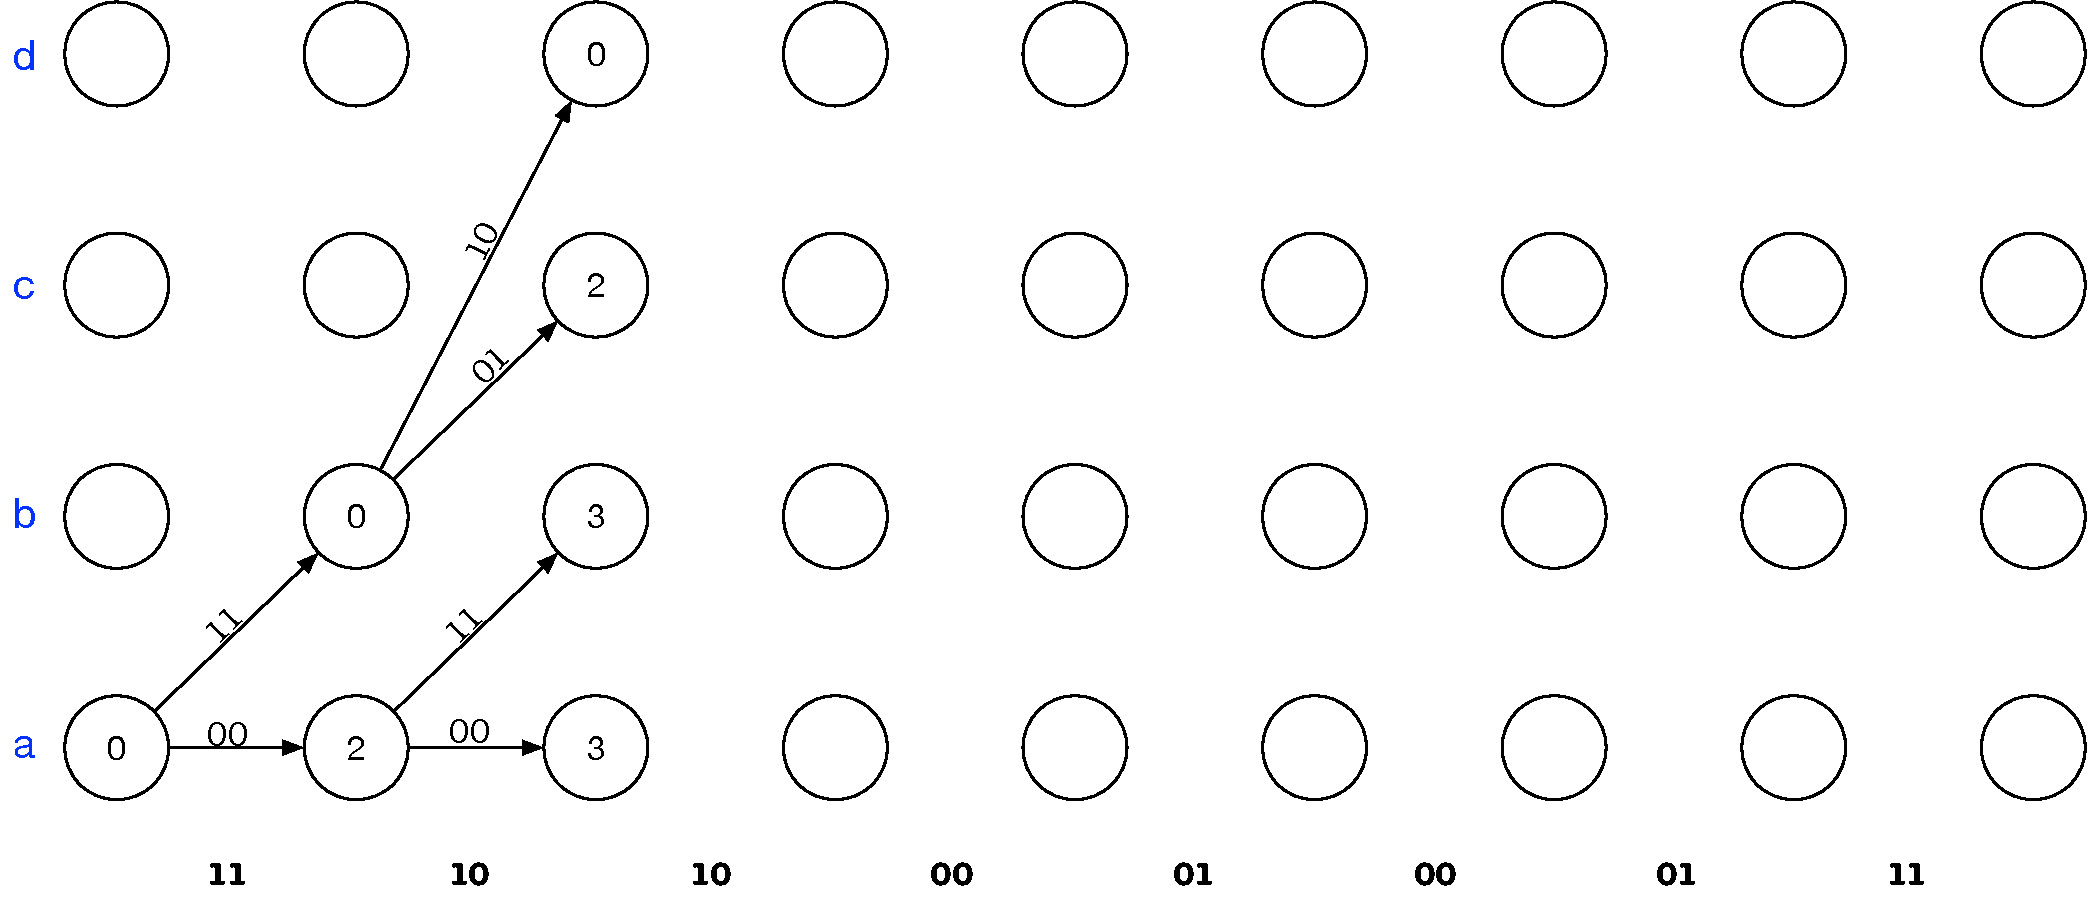
\includegraphics[width=0.8\linewidth]{Figuras/Viterbi_1.pdf}
\end{frame}

\begin{frame}{Códigos convolucionales}{Algoritmo de Viterbi}
  \centering 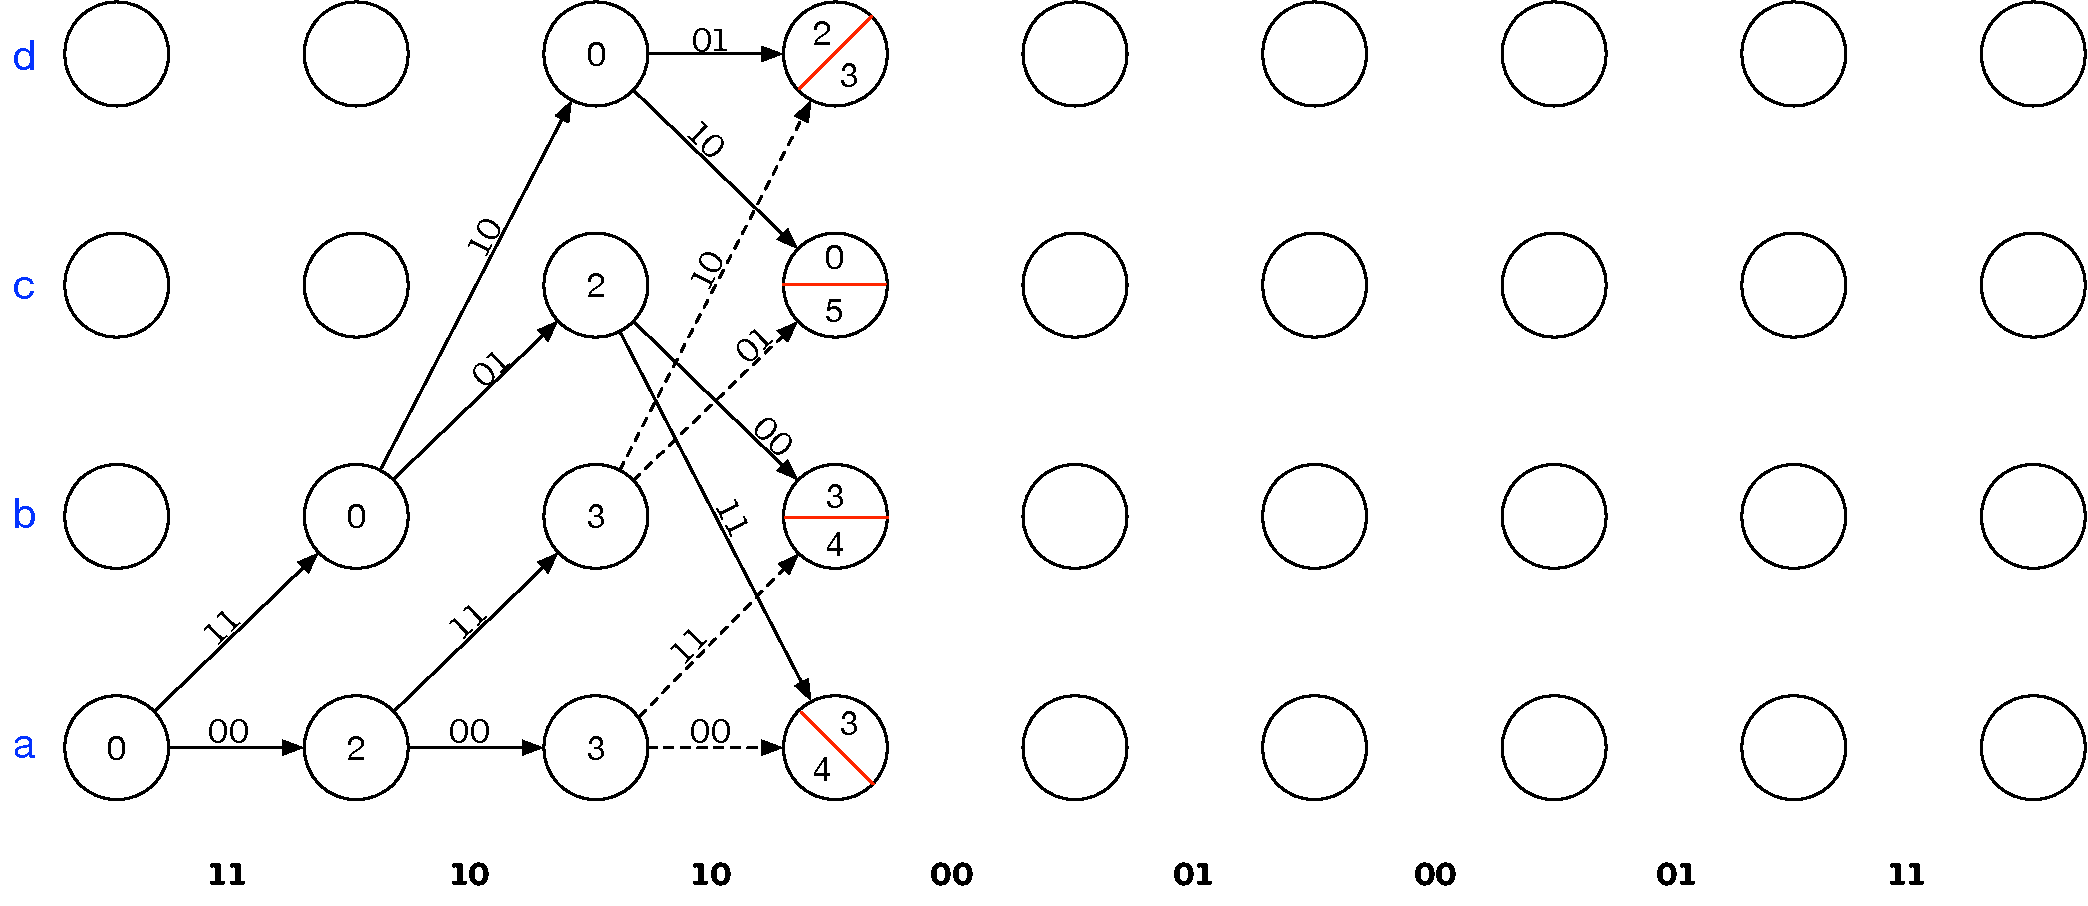
\includegraphics[width=0.8\linewidth]{Figuras/Viterbi_2.pdf}
\end{frame}

\begin{frame}{Códigos convolucionales}{Algoritmo de Viterbi}
  \centering 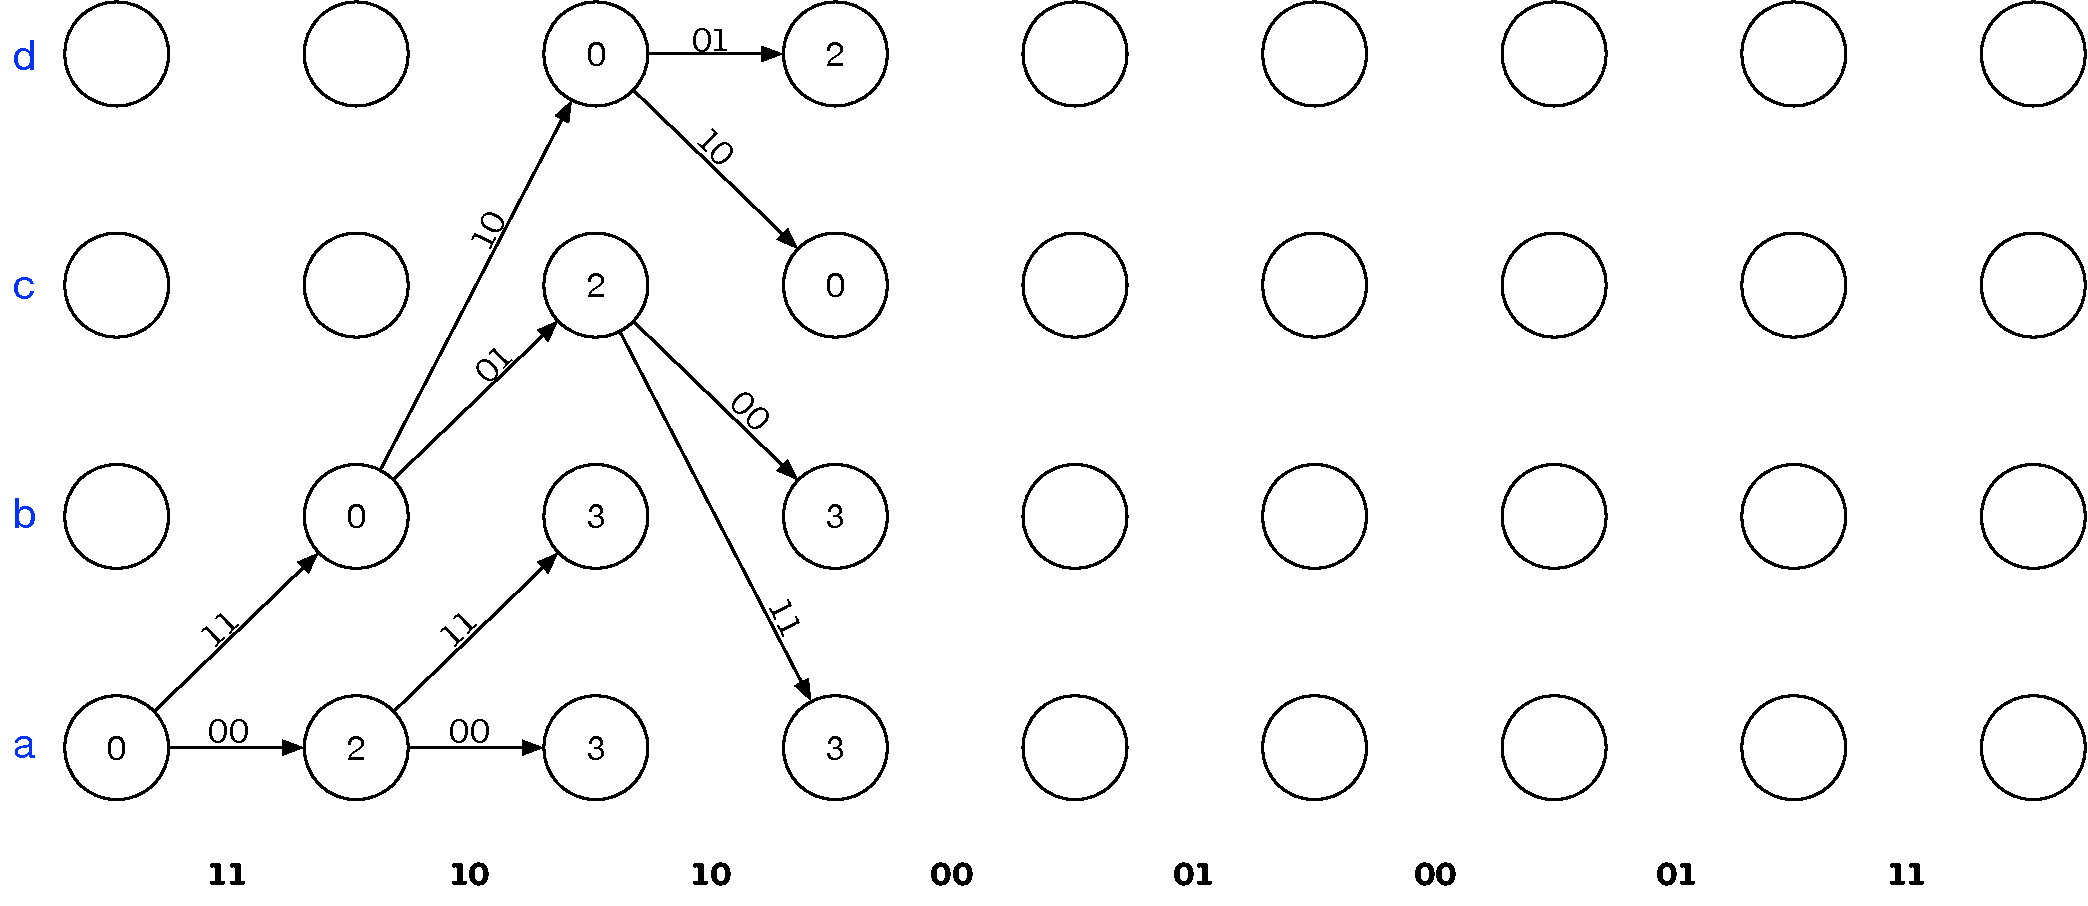
\includegraphics[width=0.8\linewidth]{Figuras/Viterbi_3.pdf}
\end{frame}

\begin{frame}{Códigos convolucionales}{Algoritmo de Viterbi}
  \centering 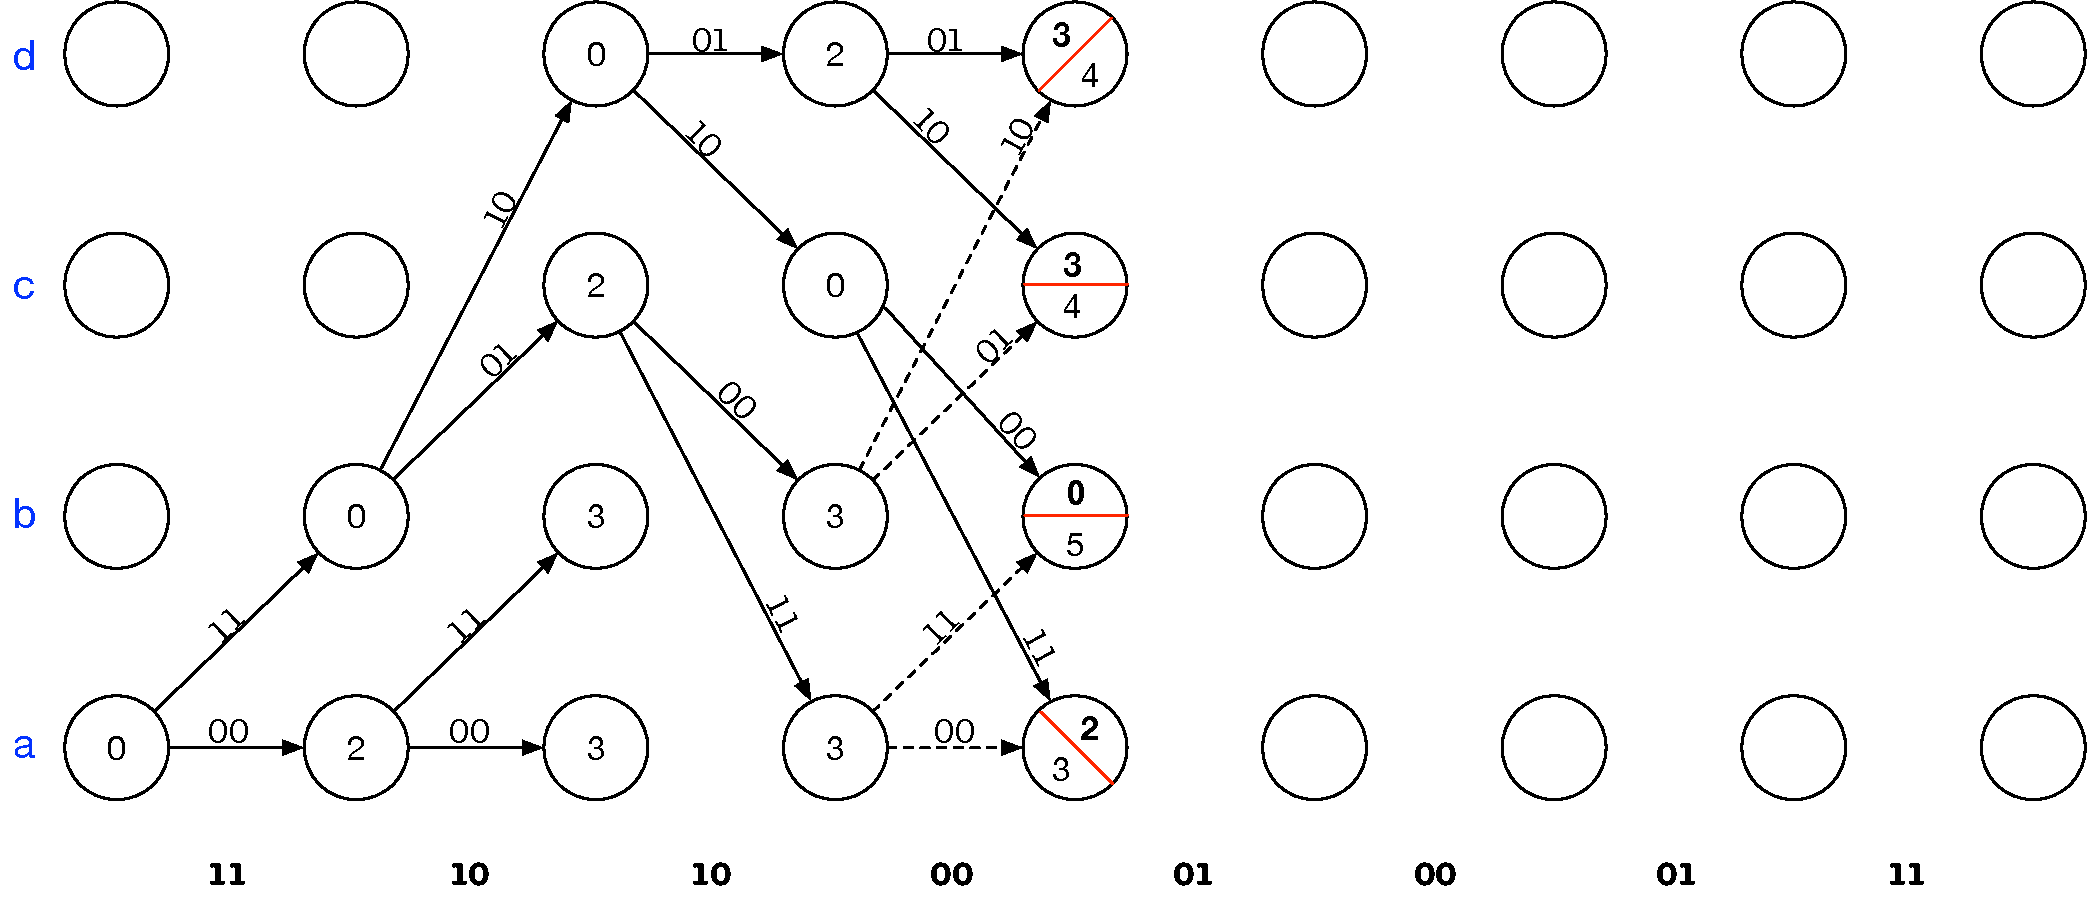
\includegraphics[width=0.8\linewidth]{Figuras/Viterbi_4.pdf}
\end{frame}

\begin{frame}{Códigos convolucionales}{Algoritmo de Viterbi}
  \centering 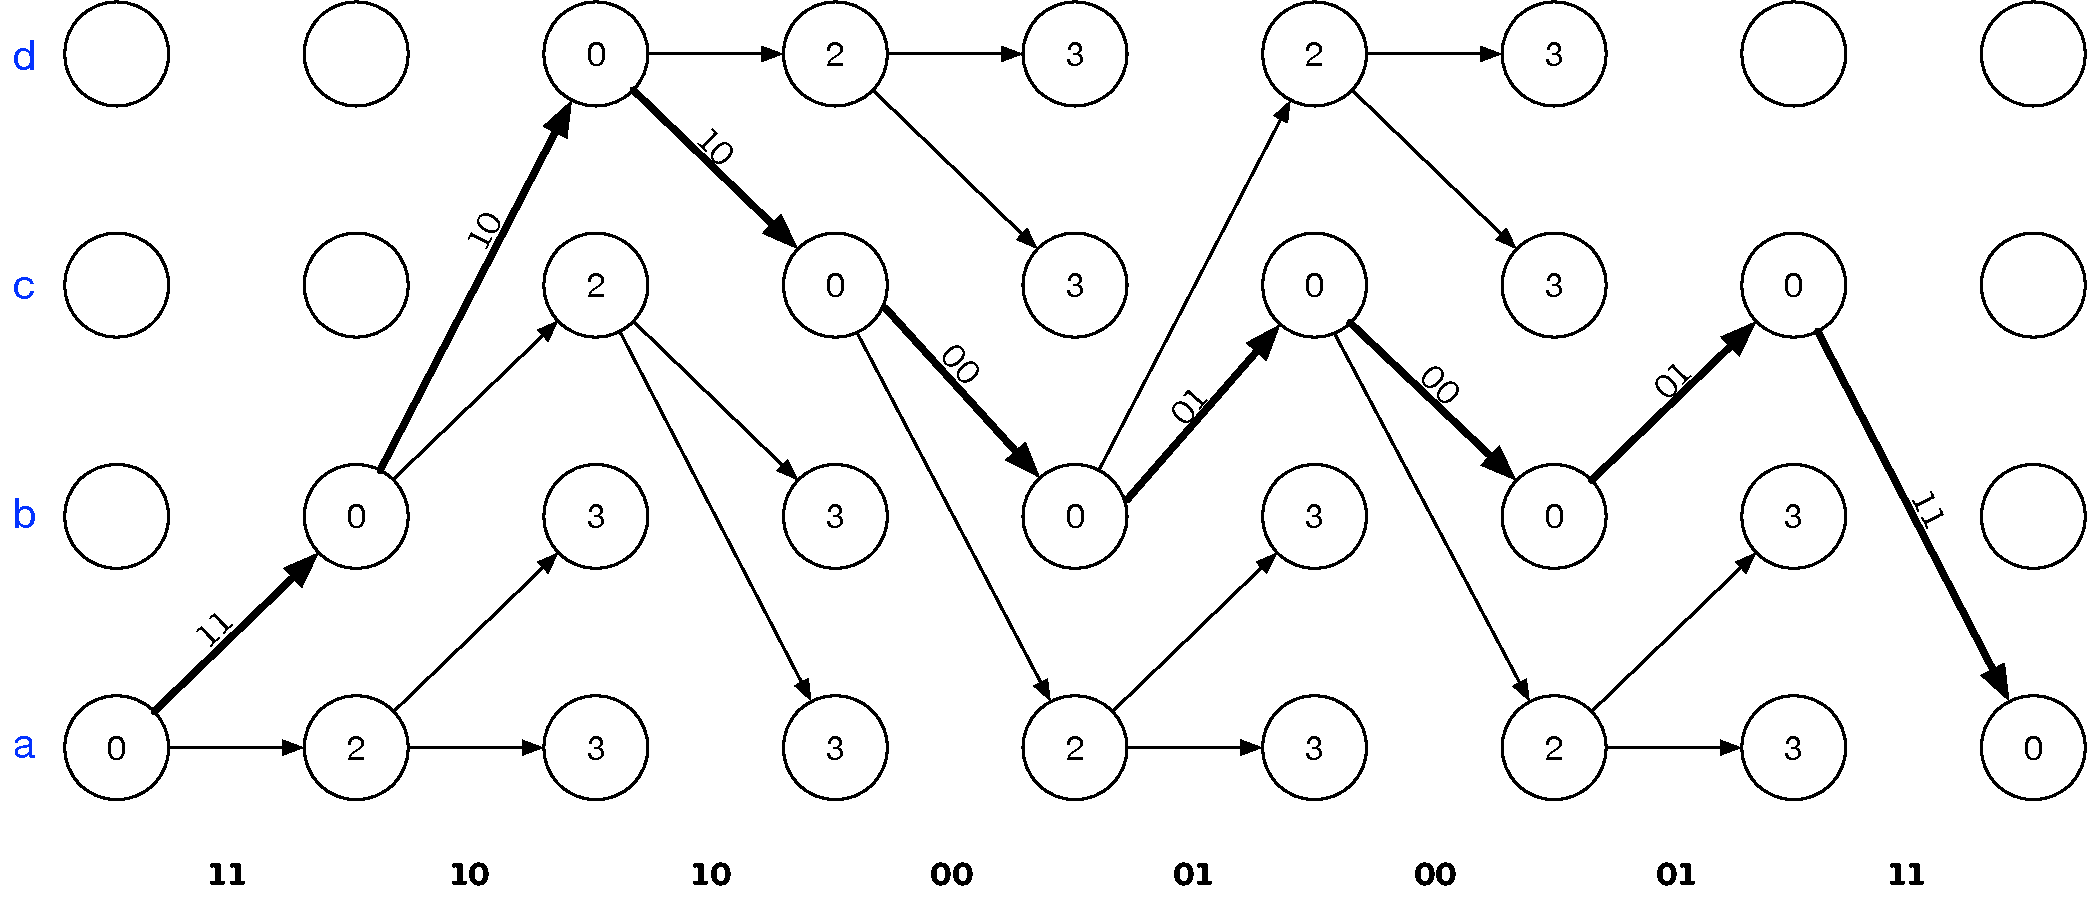
\includegraphics[width=0.8\linewidth]{Figuras/Viterbi_5.pdf}
\end{frame}



\end{document}
